\begin{figure*}[htbp]
	\centering
	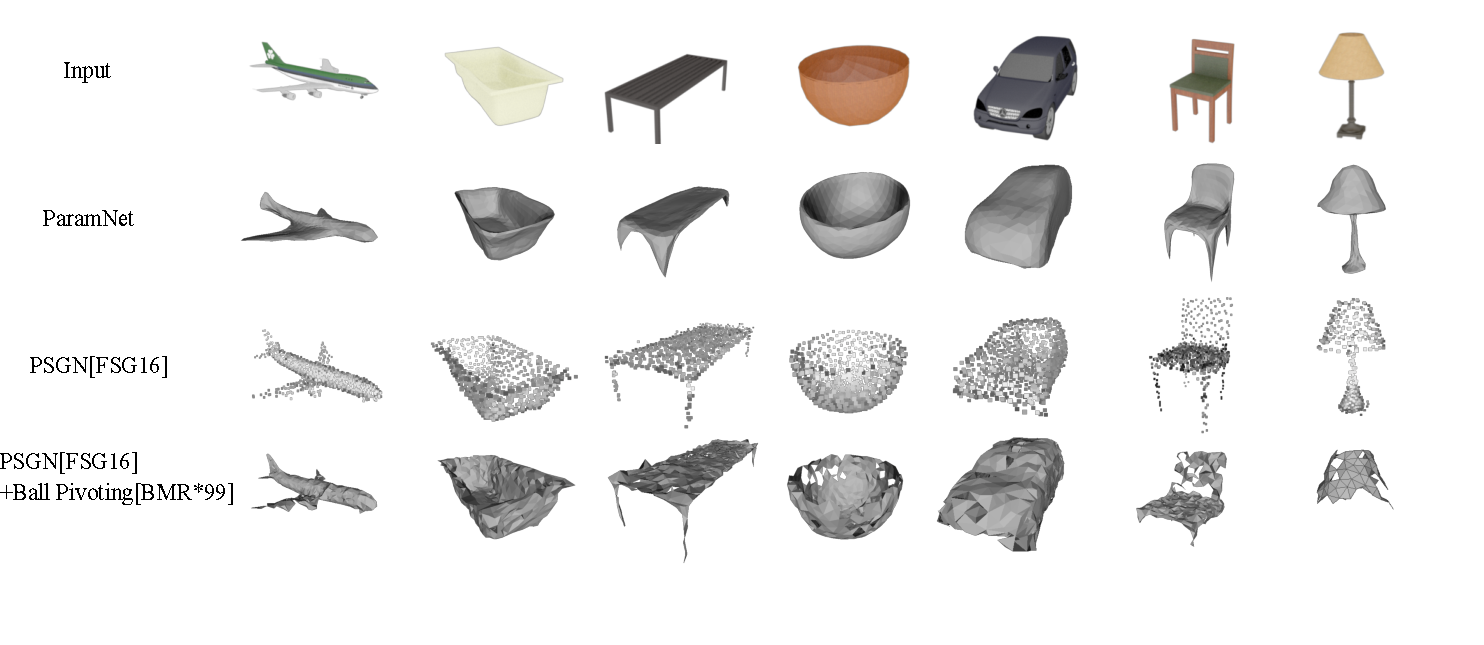
\includegraphics[width=\linewidth]{img/res/res}
	\caption{The comparison of visual results}
	\label{fig:res}
\end{figure*}
\section{Our Method}
\label{sec:net}

In this section, we first explain the general framework of our proposed network, and then we elaborate the structure details part by part.

\subsection{Network overview}
\label{subsec:overview}
Our original idea about the \emph{parameterization prediction} network was to use a semantic network that takes a single image as input to predict a mapping from the parameter domain to the target surface. 
%
%\cxj{There are five blocks/layers in our network. For each block, the semenatic network estimate a K-dimentional vector as the weights to intepolate K-neighbors. The parameterization network translates each vertex according the estimated parameters locally and then smoothes the mesh.}

In the proposed framework shown in Figure~\ref{fig:overview}, the mapping is actually expressed by the parameterization network. 
Instead of directly predicting the mapping, the semantic network predicts parameters for the parameterization network. The entire framework is end-to-end trainable.

The parameterization network is built by stacking several \textit{K}-neighbor PointNet (explained in Sec~\ref{subsec:paramnet}). 
Each \textit{K}-neighbor PointNet takes 3D point set as input and predicts a offset for each point. 
In this way, the parameterization network actually maps a randomly sampled point set to the target shape.

The semantic network is built on convolution, deconvolution and fully connected layers. It takes a single image as input to predict the parameters (i.e.$\{P_l\}$ for each layer in Figure~\ref{fig:overview}) for the parameterization network. 
In this way, the semantic network links the input image and the surface parameterization.

\subsection{Parameterization Network}
\label{subsec:paramnet}
In the proposed framework, we use unit sphere surface as parameter domain.
As shown in Figure~\ref{fig:overview}, at the beginning of the parameterization network $N=1024$ points are uniformly sampled from the parameter domain. (Here we choose $N=1024$ to be same as in \cite{PSGN}. More points can be used to express more fine details and for our framework increasing $N$ do not require the increasing of network parameter.)
Triangulation is applied on these sampled points. 
The edge connections built by triangulation are later used in the Laplacian smooth layer and the edge length regularization term. 
These connections are also used to connect output points to mesh.
 
 \begin{figure*}[htbp]
 	\centering
 	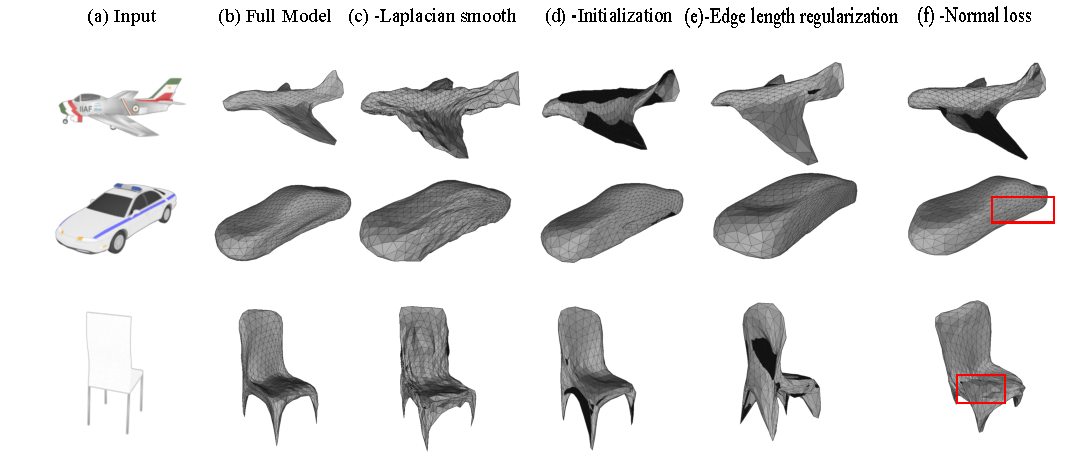
\includegraphics[width=\linewidth]{img/abl/abl}
 	\caption{Visual result for ablation study: In some cases, the view angle is adjusted for better exposure of imperfection. The black regions in the meshes are regions with flipped triangles}
 	\label{fig:abl}
 \end{figure*}
 
 \begin{table*}
 	\caption{Ablation study with respect to different components}
 	\label{tab:ablation}
 	\centering
 	\begin{tabular}{c | c c c c c}
 		Models &  Full Model & -Laplation smooth & -Initialization & -Edge length regularization & -Norm loss \\
 		\hline
 		Chamfer      & 0.297  & 0.394 & 0.424 & 0.405  & 0.390\\
 		EMD			 & 0.834  & 1.369 & 1.524 & 4.195  & 1.415
 	\end{tabular}
 \end{table*}
\noindent\textbf{\textit{K}-neighbor PointNet for parameterization network} An essential block in parameterization network is the \textit{K}-neighbor PointNet.
%
Figure~\ref{fig:knpointnet} shows its structure. 
\textit{K}-neighbor PointNet is inspired by and named after PointNet\cite{PointNet} and its follow-up PointNet++\cite{NIPS2017_7095}. 
%
In order to take unordered point set as input, \textit{K}-neighbor PointNet uses either point-wise operations on each point or symmetric functions on multiple points. 
As shown in Figure~\ref{fig:knpointnet}, the \textit{K}-neighbor search operation finds the $K$ nearest neighboring points for each point inside the $N$ input points, and outputs the indexes tensor. 
We employed the Bitonic Sort\cite{bitonicsorter} for its GPU implementation. 
Then the \emph{gather} operation re-organize the input points based on these indexes and forge the tensor of ``\textit{K}-neighbor points" as shown in Figure~\ref{fig:knpointnet}. In the tensor of ``\textit{K}-neighbor points", the coordinates of \textit{K}-neighbor
points for the $N$ input points are placed togather and results in a tensor with shape of $N\times K\times3$ 
%
The implementation for \emph{gather} operation is available in tensorflow.
Subtracting the original input points from \textit{K}-neighbor points we can get the local relative coordinates of \textit{K}-neighbor points. 
By concatenating \textit{K}-neighbor point coordinates and their local relative coordinates, we get the $N\times K\times6$ tensor as geometric features. 
%
These features go through a series of operations as shown in Figure~\ref{fig:knpointnet} to predict point-wise 3D offsets for each input point. Unlike the original PointNet\cite{PointNet}, who extracts maximum value among all point as feature vector for input point set, our \textit{K}-neighbor PointNet extract maximum value among every \textit{K}-neighborhood as feature vector for each point. This is shown by the \textit{K}-neighbor reduce max operation in Figure~\ref{fig:knpointnet}.
 
\noindent\textbf{Laplacian Smoothing}
Another essential building block for our parameterization network is the Laplacian smoothing layer. Laplacian smoothing is a traditional mesh based operation that is is commonly used in mesh processing. We integrate it into our network because most objects have locally smooth surfaces. By applying a Laplacian smoothing to the mapped/deformed surface after each \textit{K}-neighbor PointNet, we improve the visual quality of the produced mesh.

The new position of each vertex $\mathbf{x}^{*}$ in the smoothed mesh is computed as Eq.~(\ref{equ:lpl}), where $\mathcal{N}(\mathbf{x})$ represents the one-ring neighborhood of vertex $\mathbf{x}$. 
This Laplacian smoothing operation is local linear and therefore differentiable.

\begin{equation}
\mathbf{x}^* = \frac{1}{|\mathcal{N}(\mathbf{x})|}\sum_{\mathbf{y}\in\mathcal{N}(\mathbf{x})}\mathbf{y}
\label{equ:lpl}
\end{equation}

Our ablation study shows that the Laplacian smooth significantly improves the regularity of the generated surface and makes the output mesh visually more appealing.

\subsection{Semantic Network}
\label{subsec:semnet}
%
In our semantic network, we use convolution layers to extract semantic features from the input image, as shown in Figure~\ref{fig:semnet}.  
Our semantic network adopts the U-shape structure that is similar to UNet\cite{unet}. 
To fit with our parameterization framework, we use five separate decoder branches to predict different parameters for each block in our parameterization network. These predicted parameters (i.e. $P_n=\{\mathbf{W}_{n1},\mathbf{W}_{n2},\mathbf{W}_{n3},\mathbf{b}_{n3},\mathbf{W}_{n4},\mathbf{b}_{n4},s_{n}\}$ ) are plugged into the parameterization network in the way shown in Figure~\ref{fig:overview}.

\subsection{Loss Function}

The whole loss we use is defined in Eq.~(\ref{equ:loss}).
It is composed of four terms: Chamfer loss $L_{chmf}$, L2 regularization $L_{reg}$, Edge length regularization $L_{edge}$, and a normal loss $L_{norm}$.
\begin{equation}
\label{equ:loss}
L(M_p, M_g ) = L_{chmf} + L_{norm} + L_{edge}+ \alpha L_{reg}.
\end{equation}

We directly borrow the Chamfer distance from \cite{PSGN} as the Chamfer loss to measure the shape differences between the predicted mesh $M_p$ and the ground truth points $M_g$, as defined in Eq.(\ref{equ:chmf}).
%
%\noindent{\textbf{Chamfer loss}} The Chamfer distance is directly borrowed from \cite{PSGN}. This loss can drive the output point set to approach the target. As shown in Eq.(\ref{equ:chmf}). 
In Eq.(\ref{equ:chmf}), $\mathbf{x}$ are vertices on output mesh and $\mathbf{y}$ are the points from the ground truth.

\begin{equation}
\label{equ:chmf}
L_{chmf} = \sum_{\mathbf{x}\in M_p} \min_{\mathbf{y} \in M_g}||\mathbf{x}-\mathbf{y}||_2^2 + 
\sum_{\mathbf{y} \in M_g} \min_{\mathbf{x}\in M_p}||\mathbf{x}-\mathbf{y}||_2^2,
\end{equation}
where $\mathbf{x}$ are vertices of output mesh and $\mathbf{y}$ are the points from the groundtruth point clouds.

Besides of the distance of vertices, we use the {\textbf{Normal loss}} $L_{norm}$ to better guide the predicted surface to approach the groundtruth.
%, instead of emphasizing only on the approaching of output vertices, we envolve normal into our loss. 
As defined in Eq.~(\ref{equ:norm}), the $\mathbf{n}_{i}$ and $\mathbf{n}_{j}$ are the normals at vertices $\mathbf{y}_i$ and $\mathbf{y}_j$. 
$\mathbf{y}_i$ and $\mathbf{y}_j$ are respectively closest vertices to $\mathbf{x}_i$ and $\mathbf{x}_j$ in the groundtruth. 
They are found when calculating the Chamfer loss (\ref{equ:chmf}). 
This normal loss encourages the edges on the predicted meshes to remain perpendicular to the corresponding normals of its two end points.

\begin{equation}
\label{equ:norm}
L_{norm} = \sum_{(i,j)\in\mathcal{E}}\big((\mathbf{x}_i-\mathbf{x}_j)\cdot\mathbf{n}_{i}\big)^2 + \big( (\mathbf{x}_i-\mathbf{x}_j)\cdot \mathbf{n}_j\big)^2.
\end{equation}

%\noindent{\textbf{Edge Length Regularization}} 
To discourage over stretched triangles in the output mesh, we add an \textbf{Edge Length Regularization} term to minimize the variance of the edge lengths for the output mesh.
As defined in (\ref{equ:edgereg}), $\mathcal{E}$ is the set of edges, recorded as a set of paired vertex indexes (i.e. $(i,j)$).

The \textbf{L2 Regularization} loss $L_{reg}$ is applied for the parameters in our semantic network.


\begin{equation}
\label{equ:edgereg}
L_{edge} = \sum_{(i,j)\in\mathcal{E}}(\mathbf{x}_i-\mathbf{x}_j||_2 - \frac{1}{|\mathcal{E}|}\sum_{(i,j)\in\mathcal{E} }||\mathbf{x}_i-\mathbf{x}_j||_2)^2
\end{equation}



\subsection{Training} 
\noindent \textbf{Dataset.}
%%===data===%%
We train and evaluate our models on the ShapeNet\cite{shapenetdata}. Specifically, we use the ShapeNetCore55.v2 which contains over 50k manually created and cleaned 3D CAD models in 55 category.
The images for training and testing are rendered in 16 random angles to provide synthetic training data for the model. 
In total, 51,856 shape models are covered. 
For the training/validation/testing split, we follow the CSV file provided by the ShapeNet website and resulted in 36,622/5,110/10,124 shapes. 
The 3D CAD objects are stored as meshes, and we re-sample the meshes into point sets. 
In order to capture only the shape surface, we uses the code from~\cite{ocnn} and execute ``virtual scan" for the re-sampling.
For each view angles, we sample 2 different point samples as ground truth for training and testing. In other words, for each CAD model we generate 32 pairs of image and point set as our data in training/validation/testing.

\noindent \textbf{Network Super Parameters}
Unless otherwise stated, the network super parameters are chosen as follows for implementation of our framework presented in this paper. We use four \textit{K}-neighbor PointNet, whose $K=16$. 

\noindent \textbf{Network Initialization}
Even with the well-designed loss functions, the proposed network might output surfaces with severe global self-intersection, when we train it from scratch.
%
To alleviate this problem, we adopt a \emph{network initialization} step to reset the parameterization network to start from a state that produce surface without self-intersection. In other words, for any input image, we first expect the network to map the parameter domain to a smaller sphere surface (radious=0.5), instead of predicting a shape to approach the ground truth.
Thus, the loss function for this initialization step is defined as:
\begin{equation}
\label{equ:init}
L_{init} = \sum_{\mathbf{x}\in M_p}\min_{\mathbf{y}\in S_{0.5}}||\mathbf{x} - \mathbf{y}||_2^2.
\end{equation} 
%The $\mathbf{y}$ used in Eq.(\ref{equ:init}) is not the points from groundtruth, but the points sampled from parameter domain with a 0.5 scale down. 
%In other words, this step will reset the network so that the parameterization network will map from a sphere to a smaller sphere, when taking any image as input. 
We do this training of initialization by one epoch on the training data. 

\noindent \textbf{Training configuration}
Unless otherwise stated, our networks are trained with following configurations.
We use Adam optimizer\cite{adam} with learning rate of $3e-5$. We use $\alpha=1e-5$ for training loss.  
We use 32 as size for mini-batch. For each training iteration, we re-sample $N=1024$ points from the parameter domain and do triangulation with them. These sampled points are shared inside a mini-batch and therefore triangulation is also shared across the mini-batch.  For comparison, our network and \cite{PSGN} are both trained 8 epochs on the training data.
Typically, it takes four and a half day to train our network on 4 Tesla K80. 

\begin{figure}[htbp]
	\centering
	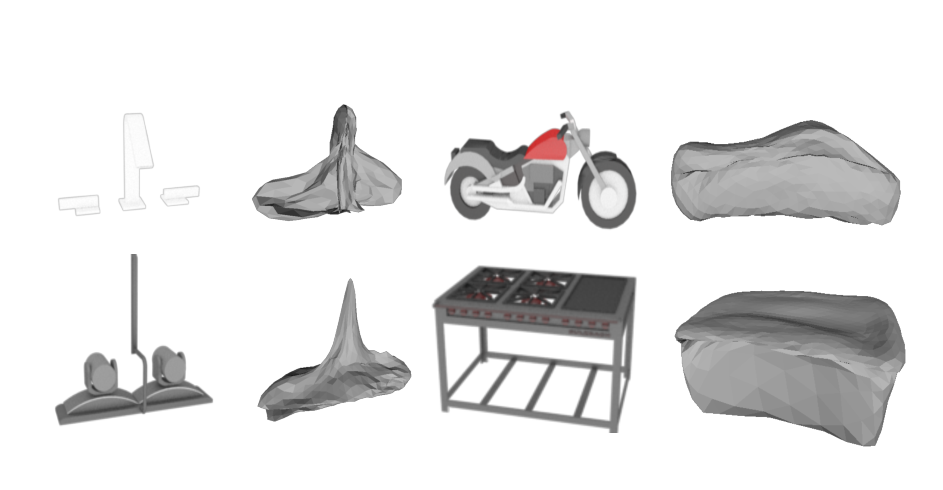
\includegraphics[width=\linewidth]{img/fail/fail1}
	\caption{Failure cases: In some cases, the view angle is adjusted for better exposure of imperfection}
	\label{fig:fail1}
\end{figure}
\begin{figure}[htbp]
	\centering
	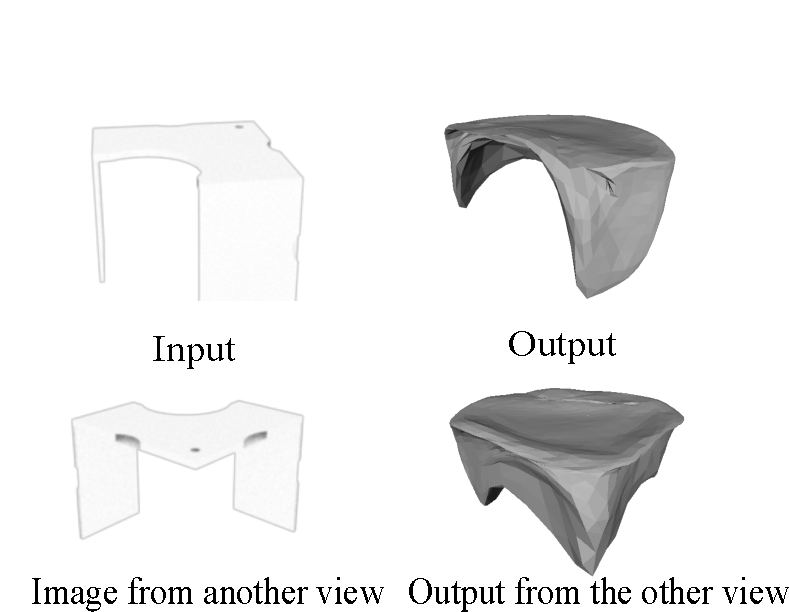
\includegraphics[width=\linewidth]{img/fail/fail2}
	\caption{Failure case: In this case, the network have output an extra leg that doesn't exist for the dresser}
	\label{fig:fail2}
\end{figure}
\begin{table}
	\caption{Ablation study with respect to number of \textit{K}-neighbor PointNet}
	\label{tab:pointnet}
	\centering
	\begin{tabular}{c | c c c c}
		Number of \textit{K}-n PointNet &  2 & 3 & 4 & 5 \\
		\hline
		Chamfer      & 0.425 &  0.411 & 0.297 & 0.313 \\
		EMD			 & 1.304 &  1.360 & 0.834 & 1.067 \\
		\hline
		Training Time& 3d20h &   4d2h   & 4d10h & 4d23h
	\end{tabular}
\end{table}


